% section 3: Models and evaluation method (precision and recall). Comparision among models by f1-score method (show some plots of the main results)
\section{Models}

We tried the following different models:
\begin{enumerate}
	\item Custom Inception Net: a custom version of the Inception\_v1 network;
	\item Custom Resnet: a custom version of the Resnet 101;
	\item Resnet50 (pretrained).
\end{enumerate}

Each model can be found in the directory \texttt{models}.
For each model we will show the comparison between validation and training loss. The final models (which are saved in the directory) are chosen when the validation error is lowest in order to avoid overfitting and get the most general solution.

\subsection{Custom Inception Net}

\begin{figure}[!h]
	\begin{center}
		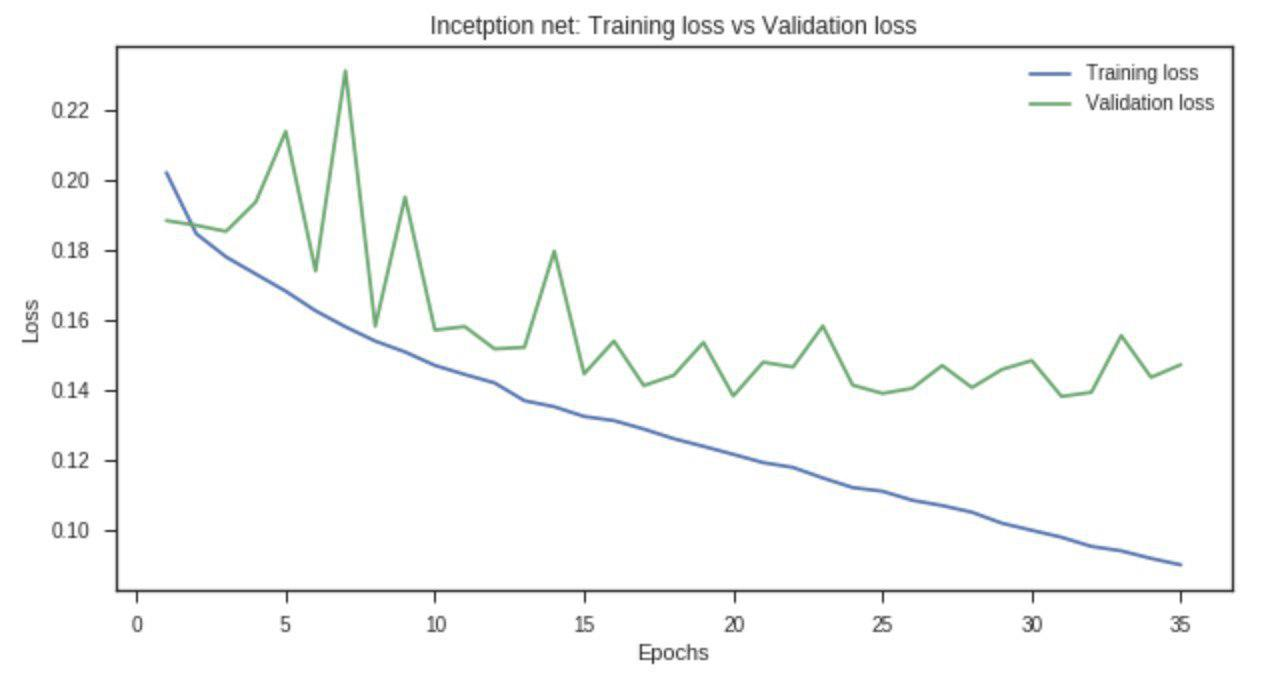
\includegraphics[width=0.6\linewidth]{images/custom_inception_loss.jpg}
		\caption{Custom Inception Net loss}
		\label{fig:cust-incep-loss}
	\end{center}
\end{figure}


%\begin{center}
%	\begin{tabular}{ l | c | c | r }
%		\hline
%		\textbf{Model} & \textbf{accuracy} & \textbf{recall} & \textbf{f1-score}  \\ \hline
%		Inception\_v1 & & & \\
%		Resnet101 & & & \\
%		Inception\_v2 & & & \\
%		\hline
%	\end{tabular}
%\end{center}